\documentclass{beamer}
\usepackage{amsmath}
\usepackage{amssymb}
\usepackage{pgf}
\usepackage{tikz}
\usetikzlibrary{matrix}
\usetheme{boxes}
\newcommand{\fig}{figures}
\newcommand{\frnzplt}{FranzPlot }
\title{Proiezioni ortogonali di solidi, esercizio}

\begin{document}

\begin{frame}
\maketitle
\end{frame}
\begin{frame}
\frametitle{Consegna}
Disegnare con povray l'insieme di oggetti mostrato dalle seguenti proiezioni ortogonali.
\end{frame}
\begin{frame}
\frametitle{Proiezione piano x-y}
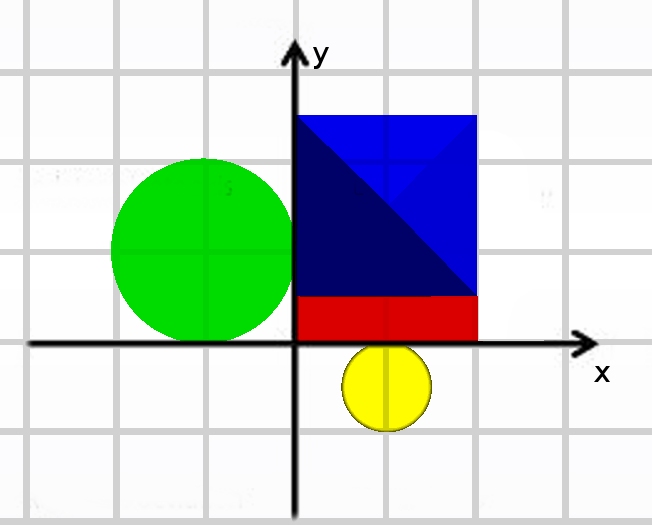
\includegraphics[width=0.9\textwidth]{\fig/proj1.png}
\end{frame}
\begin{frame}
\frametitle{Proiezione piano x-z }
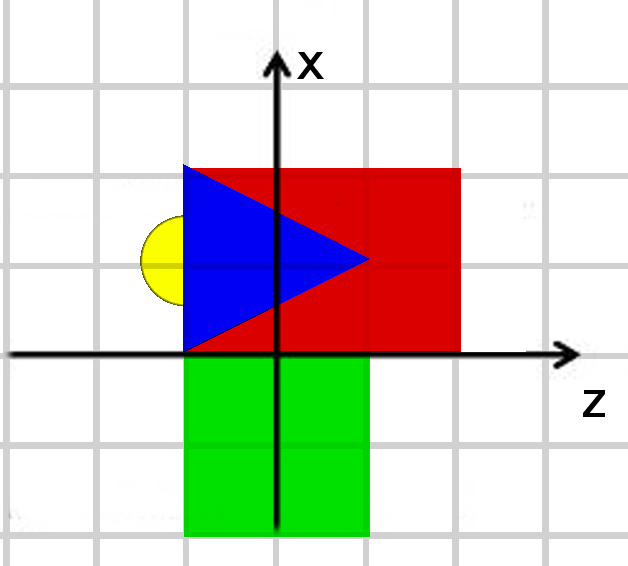
\includegraphics[width=0.9\textwidth]{\fig/proj2.png}
\end{frame}
\begin{frame}
\frametitle{Proiezione piano y-z}
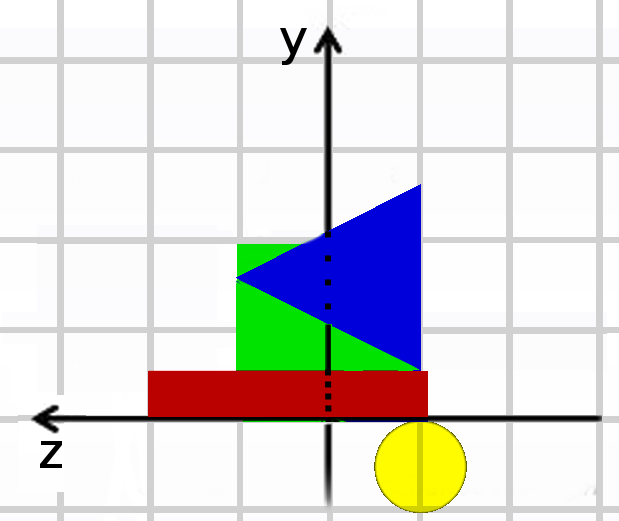
\includegraphics[width=0.9\textwidth]{\fig/proj3.png}
\end{frame}
\begin{frame}
\frametitle{Oggetti}
Dalle tre figure precedenti si identificano:
\begin{enumerate}
\item Sfera (Gialla) di raggio 0.5 centrata in (1,-0.5,-1) 
\item Prisma retto a base rettangolare (Rosso), definito dai vertici 
(0,0,-1),(2,0,-1),(2,0.5,-1),(0,0.5,-1),
(0,0,2) ,(2,0,2) ,(2,0.5,2) ,(0,0.5,2)
\item Piramide retta a base quadrata (Blu) con vertici della base in (0,0.5,-1), (2,0.5,-1), (2,2.5,-1) e (0,2.5,-1) ed apice in (1,1.5,1).
\item Cilindro circolare retto (Verde) con base di raggio 1 ed altezza parallela a z. I centri delle due basi sono rispettivamente in (-1,1,-1) e (-1,1,1).
\end{enumerate}
\end{frame}
\begin{frame}
\frametitle{Grafi - Sfera}
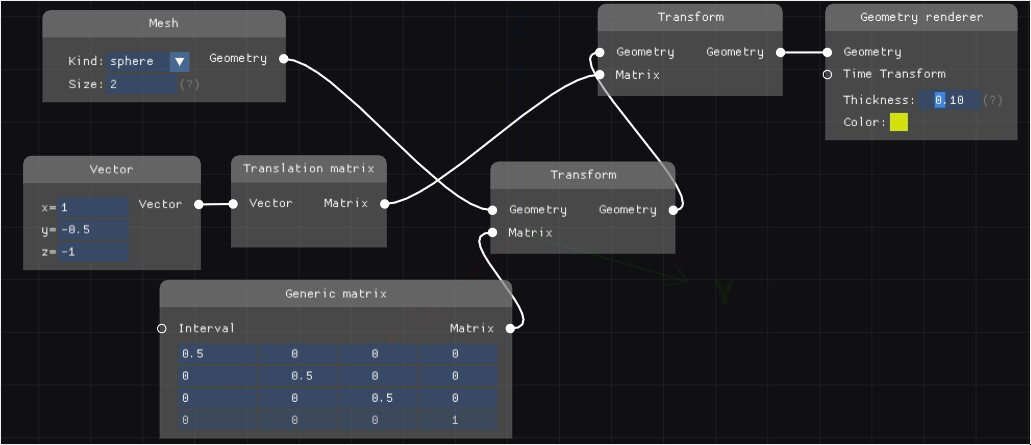
\includegraphics[width=\textwidth]{es_solidi_graph_sphere.jpeg}
\end{frame}
\begin{frame}
\frametitle{Grafi - Sfera}
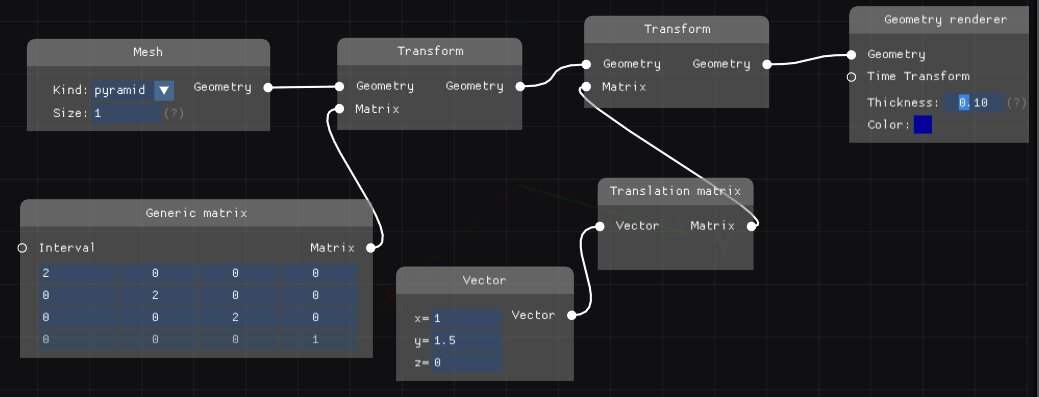
\includegraphics[width=\textwidth]{es_solidi_graph_pyramid.jpeg}
\end{frame}
\begin{frame}
\frametitle{Grafi - Sfera}
\includegraphics[width=\textwidth]{orth-sol.jpg}
\end{frame}
\begin{frame}
\frametitle{Grafi - Sfera}
\includegraphics[width=\textwidth]{orth-sol.jpg}
\end{frame}
\begin{frame}
\frametitle {Oggetti}
\includegraphics[width=\textwidth]{orth.pdf}
\end{frame}
\end{document}
